% !TeX document-id = {4002cb99-008b-434a-ab42-cf6c5ca92d10}
% !TeX encoding = UTF-8
% !TeX program = pdflatex
% !BIB program = biber
%%% To write an article in English, please use the option ``english'' in order
%%% to get the correct hyphenation patterns and terms.
%%% \documentclass[english]{class}
%%% for anonymizing an article you can use the ``anonymous'' option.
%%%
%%% Um einen Artikel auf deutsch zu schreiben, genügt es die Klasse ohne
%%% Parameter zu laden.
%%% Zur Anonymisierung kann die ``anonymous'' Option genutzt werden.
\documentclass[english]{lni}
%%
\addbibresource{mybibfile.bib}
%\renewcommand{\refname}{References}
\usepackage{draftwatermark}
\usepackage[]{draftwatermark} % nur erste Seite
\usepackage{graphicx}
\usepackage{subcaption}
\usepackage{float}
\graphicspath{{images/}}
\SetWatermarkText{Autonomous Systems - Summer Term 2026}
\SetWatermarkLightness{0.98}            % etwas dunkler als default
\SetWatermarkScale{0.25}                  % default scale: 1.2
\begin{document}
%%% Mehrere Autoren werden durch \and voneinander getrennt.
%%% Die Fußnote enthält die Adresse sowie eine E-Mail-Adresse.
%%% Das optionale Argument (sofern angegeben) wird für die Kopfzeile verwendet.
\title[Truck Platooning]{Truck Platooning: SVM-Based Line Following and Formal Verification with Timed Automata - Team 5}
\author[Odaudu, Chowdhury, Qaiser]{%
	Iko-ojo Victor Odaudu\footnote{\email{iko-ojo-victor.odaudu@stud.hshl.de}}
	\and Hany Chowdhury\footnote{\email{hany.chowdhury@stud.hshl.de}}
	\and Muhammad Mujhtaba Qaiser\footnote{\email{muhammad-mujhtaba.qaiser@stud.hshl.de}}%
}
\startpage{1} % Beginn der Seitenzählung für diesen Beitrag / Start page
\booktitle{} % Name of book title
\maketitle

{\setcounter{tocdepth}{1}\tableofcontents}
\bigskip

\section{Motivation}
\textit{Written by: Muhammad Mujhtaba Qaiser}
\\~\\
Truck platooning is the idea of letting trucks drive close together in a convoy, with a leader truck in front and one or more follower trucks behind it that basically copy what the leader does. This is interesting because it can save fuel, since the trucks behind sit in the slipstream of the one in front, and it can also make better use of the road. The systems engineering side of building something like this is well described in references like the INCOSE Systems Engineering Handbook, which is why we treated the project as a proper engineering task with requirements, models and checks instead of just writing code.

The hard part is safety. A follower truck that drives itself has to keep a safe distance, stay in its lane, and react correctly when something goes wrong, like the wireless link dropping or an obstacle suddenly appearing. Because of that we did not only build the driving software, we also modelled the important situations formally and proved that the system reacts the way it should. This report goes through both parts: the machine learning that keeps the follower on the line, and the formal models that show the whole thing behaves safely.

\section{SVM-Based Line Following}
\textit{Written by: Iko-ojo Victor Odaudu (training), Muhammad Mujhtaba Qaiser (data gathering from the truck), Hany Chowdhury (testing)}
\\~\\
The machine learning part of the project is the bit that keeps the follower truck on the line. The line is painted green on the road, and the truck has a camera that gives us one frame at a time. So our job was basically to take what the camera sees and turn it into a steering value the truck can actually use. Camera-based line following like this builds directly on the material we covered in our lab classes earlier in the semester, where we worked through image processing and simple classifiers step by step. The whole pipeline we describe here is implemented in our own lab notebook.

\subsection{Feature and Approach}
Instead of feeding the whole image into a model, we reduce each frame down to a single number that we call the offset. We take the lower part of the camera image, because that is the part of the road closest to the truck and the most relevant for deciding how to steer right now, then we mask out the green pixels of the line and find where the centre of the line is compared to the middle of the image. To pull out the green pixels we work in the Hue, Saturation, Value (HSV) colour space and threshold on the green range, which is the standard way of doing colour masking and something we had already practised in the lab classes. That gives us one value between $-1$ and $+1$, where a negative number means the line is off to the left and a positive number means it is off to the right. After that we smooth this offset over the last few frames using a running median, so that one single noisy frame does not throw off the steering and cause the truck to jerk around.

For the model itself we use a Support Vector Machine (SVM), which is a model that learns to separate classes by finding good boundaries between them, and which we had already seen and used in the lab classes. We went with an SVM because our input is just one clean feature, so we did not really need something heavy like a neural network, and an SVM trains quickly and is pretty easy to reason about. The model was built as a pipeline with feature scaling first and then the SVM, and the settings were tuned automatically with a grid search that used cross validation, so the choice of kernel and parameters was not just something we guessed.

\subsection{From Three Classes to Five, and the Controller}
At the start we only used three classes, which were left, straight and right. The problem was that this steered too roughly, since a slight curve and a sharp curve were being treated the exact same way. To fix that we moved up to five classes, going from hard left, soft left, straight, soft right, to hard right. This lets the truck react gently on the small curves and more strongly on the sharp ones, which makes the driving a lot smoother.

The SVM does not steer the truck directly on its own. It works together with a controller that takes the situation and turns it into a smooth steering command, so the truck corrects gradually instead of jerking left and right. The five classes also do real work here, because when the model detects a hard turn the steering is pushed harder than it would be for a soft turn. On top of that we smooth the final steering value over time so the driving stays stable. The whole thing runs live on the truck, which we set up in the same way as in the lab classes, so it reads each camera frame, works out the offset, predicts the class, and sends out a steering command in real time.

\section{Dataset and Evaluation}
\textit{Written by: Iko-ojo Victor Odaudu}
\\~\\
We collected our data from the ScienceTruck, and on top of that we also generated some synthetic line images to add more examples to work with. The five classes come from labelling each sample by its offset, going from hard left all the way to hard right.

The main issue we ran into was that the dataset was very unbalanced. On a normal track the truck drives straight most of the time, so we ended up with a huge number of straight samples, over twenty thousand of them, but only around a hundred samples for the hard turns. When we trained the SVM on this raw data, it basically learned to always predict straight, because that was the correct answer most of the time anyway. It still looked accurate on paper, but it was pretty much useless for actually steering through turns, and this was the point where the model kept getting the turns wrong, which are the cases that actually matter. The class counts before and after balancing are shown in Figure~\ref{fig:classdist}.

\begin{figure}[H]
	\centering
	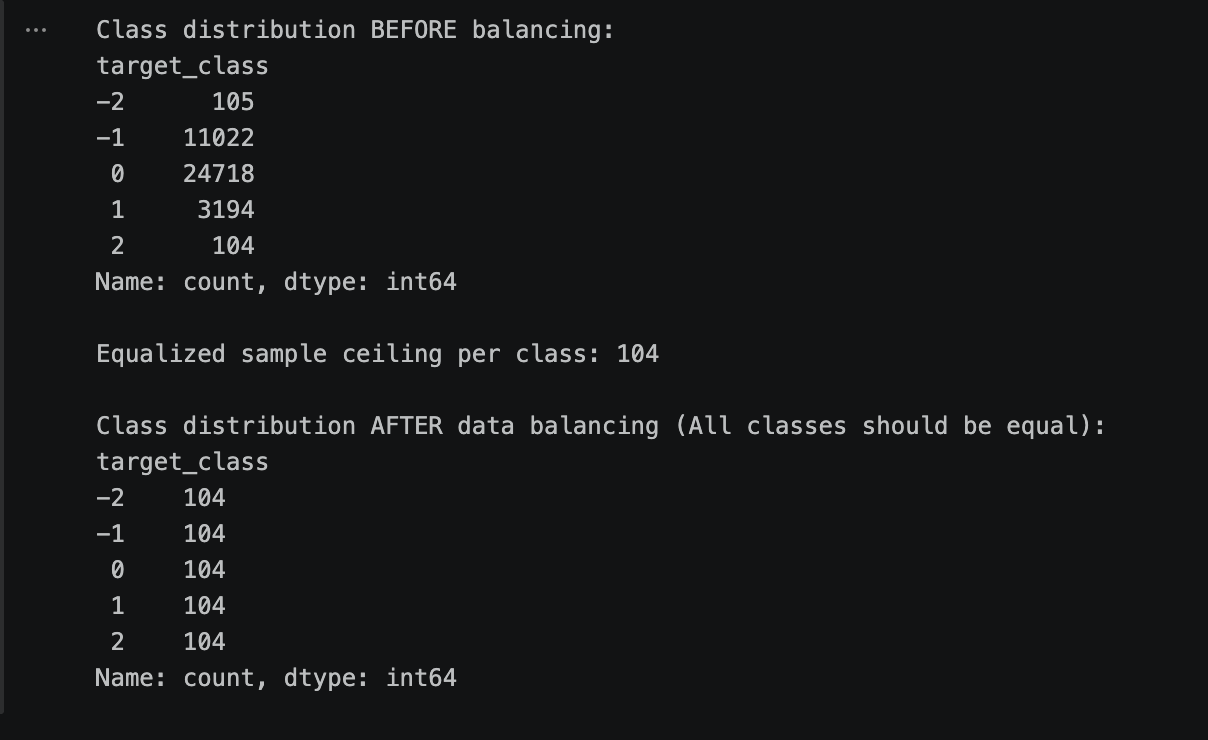
\includegraphics[width=0.52\textwidth]{class_distribution.png}
	\caption{Class distribution before and after balancing. The raw data is dominated by the straight class (over 24{,}000 samples) while the hard turns only have around 100, so every class is cut down to the size of the smallest one (104 samples) before training.}
	\label{fig:classdist}
\end{figure}

To fix this we balanced the dataset by cutting every class down to the size of the smallest one, which was about 104 samples per class. This is a random undersampling approach, which is one of the standard ways of dealing with an imbalanced dataset and something the lab classes had pointed us to. That way all five directions are represented equally and the model is forced to actually learn the turns instead of taking the easy way out. After balancing, the model reached about 99\% accuracy on the test set. The classification report and confusion matrix in Figure~\ref{fig:eval} show the result, with high precision and recall across all five classes and almost everything sitting on the diagonal of the matrix, which basically means the model rarely mixes up one direction for another. The only mistake is a single sample that got confused between hard left and soft left.

\begin{figure}[H]
	\centering
	\begin{subfigure}[t]{0.48\textwidth}
		\centering
		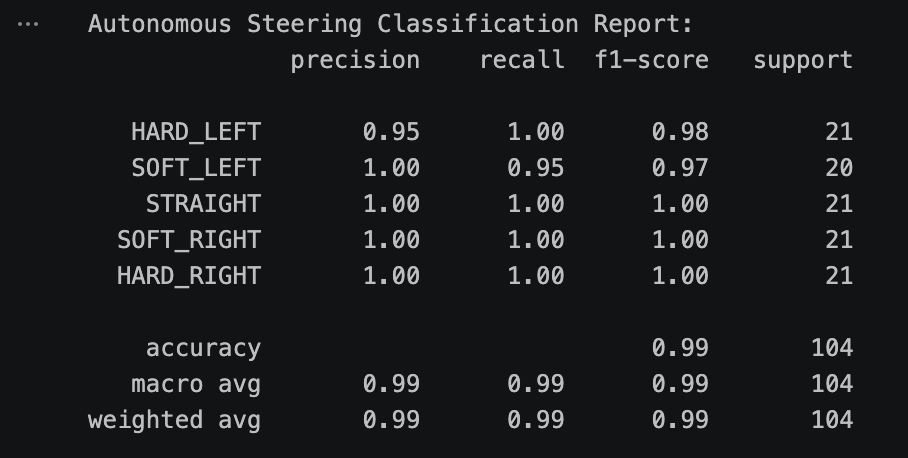
\includegraphics[width=\textwidth]{classification_report.png}
		\caption{Classification report.}
		\label{fig:report}
	\end{subfigure}
	\hfill
	\begin{subfigure}[t]{0.48\textwidth}
		\centering
		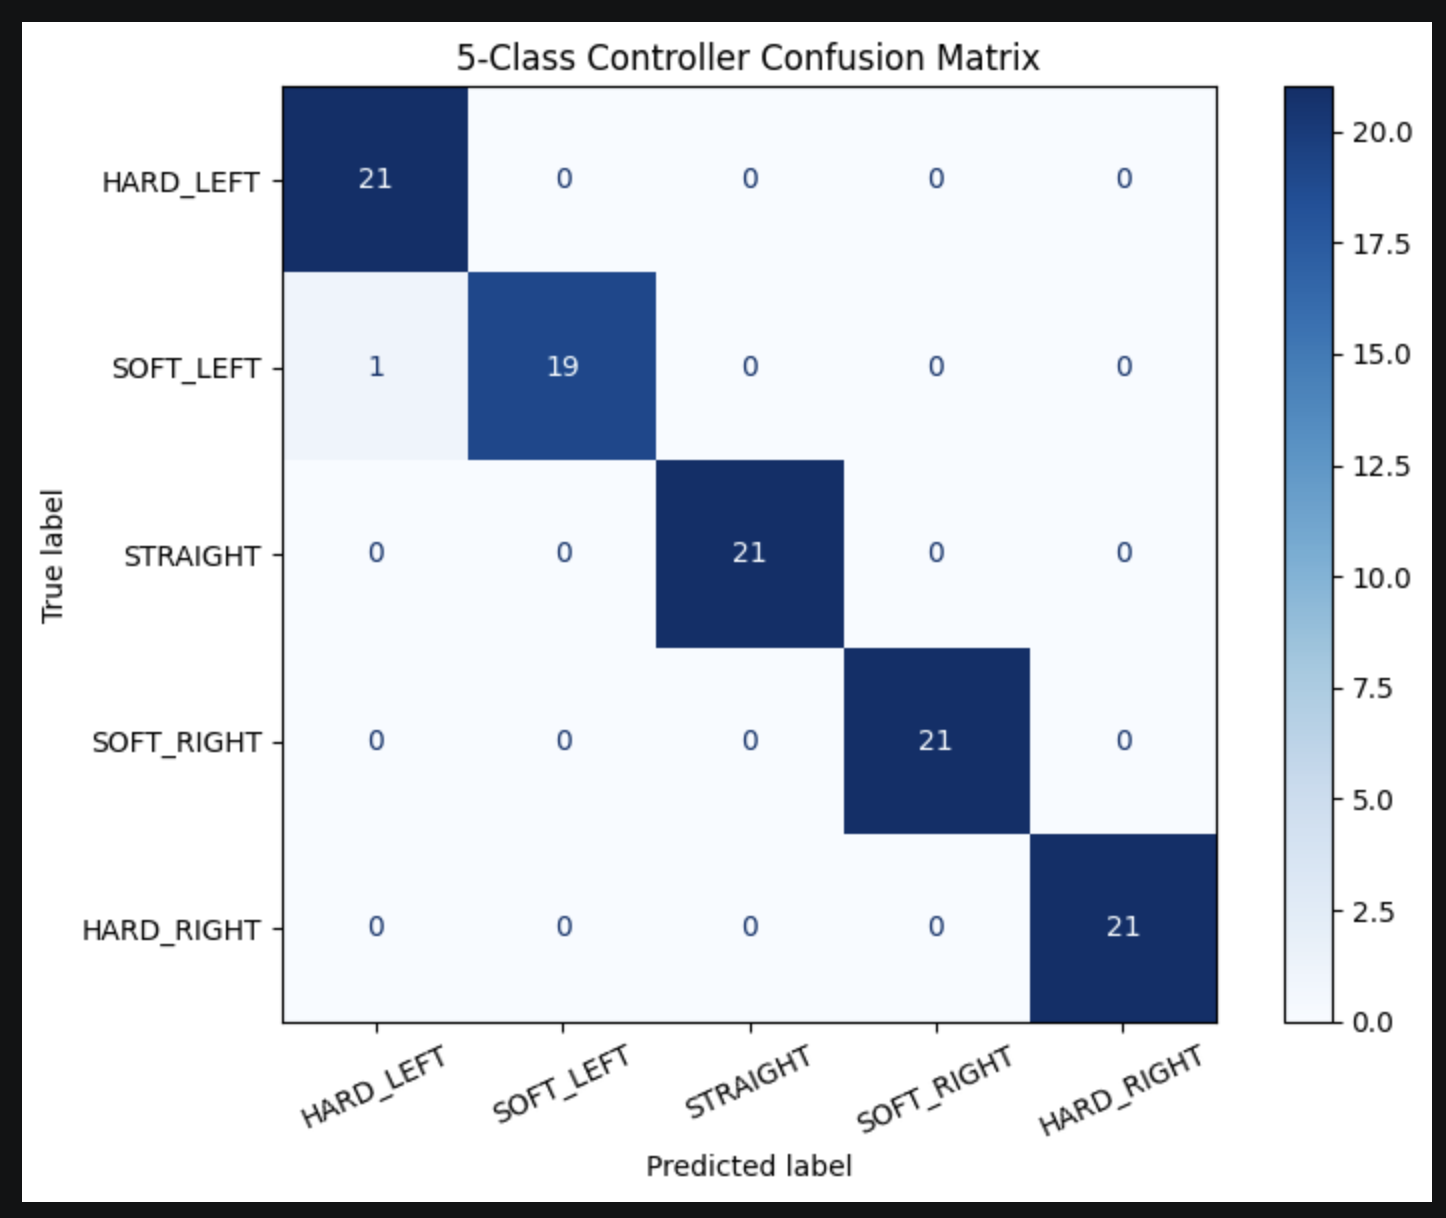
\includegraphics[width=\textwidth]{confusion_matrix.png}
		\caption{Confusion matrix.}
		\label{fig:confusion}
	\end{subfigure}
	\caption{Evaluation on the balanced test set (104 samples). The classification report shows high precision and recall for every class, and almost all of the predictions in the confusion matrix sit on the diagonal, so the model classifies the steering direction correctly nearly every time. The only mistake is one sample confused between hard left and soft left.}
	\label{fig:eval}
\end{figure}

\section{Scenario Descriptions and Requirements}
\textit{Written by: Iko-ojo Victor Odaudu, Hany Chowdhury, Muhammad Mujhtaba Qaiser (one scenario each)}
\\~\\
We looked at three scenarios, and each of us took responsibility for one of them. Together they cover normal driving, a communication problem, and an emergency. For each scenario we wrote down the data, signals and events that the trucks need to exchange, who sends them and who receives them, and the timing that has to be met.

\subsection{Scenario 1: Normal Platooning}
In normal platooning everything is working the way it should. The leader keeps sending its speed and position, and the follower stays in its lane using the camera while also keeping a safe distance. The main requirements here are that the leader sends its speed and position at least every 100\,ms, that each camera frame is processed within 33\,ms (which comes from running the camera at 30 frames per second), and that a steering correction is applied within the same frame. On the safety side, if the gap to the leader drops below 5\,m the follower reduces speed automatically, it never drives faster than the leader, and if the lane markings are lost for more than three frames it slows down and raises an alert.

\subsection{Scenario 2: Communication Failure}
Here the wireless link drops and the follower stops receiving beacons from the leader. The follower has to notice this on its own and then react safely. The requirement is that it detects the failure within 500\,ms of the last message, switches into a fallback mode within 100\,ms of detecting it, and starts slowing down smoothly instead of braking hard. While all this is happening the camera keeps doing lane keeping, so the truck stays in its lane even without the leader's data. If the link comes back before 10 seconds the follower goes back to normal platooning, and if it does not, the follower comes to a full stop at 10 seconds.

\subsection{Scenario 3: Emergency Braking}
In this scenario an obstacle suddenly appears ahead of the leader, so the leader brakes hard and sends a brake signal to the follower. The important idea here is that neither the wireless link nor the camera should be a single point of failure, so there are three paths. In Path A the brake signal arrives and the follower brakes within 200\,ms. In Path B the signal is missed, but the camera sees the leader slowing down and braking is triggered within 300\,ms. In Path C, if neither path has caused braking within 400\,ms, the follower does a precautionary controlled stop just to be safe. In all cases the braking stays smooth and the truck stays in its lane.

\section{SysML/UML Models}
\textit{Written by: Hany Chowdhury}
\\~\\
To describe how the trucks and their parts talk to each other in each scenario, we modelled the three scenarios as sequence diagrams. A sequence diagram is useful here because it shows the order of messages over time between the different parts, things like the leader truck, the wireless link, the follower truck, the camera and lane detection, the controllers and the actuators. Each arrow is a message or a signal, and the timing constraints from the requirements are written next to the arrows they belong to, so you can see the deadlines right where they apply. The three diagrams are shown in Figure~\ref{fig:seq}, and we go through each one briefly below.

\begin{figure}[H]
	\centering
	\begin{subfigure}[t]{0.32\textwidth}
		\centering
		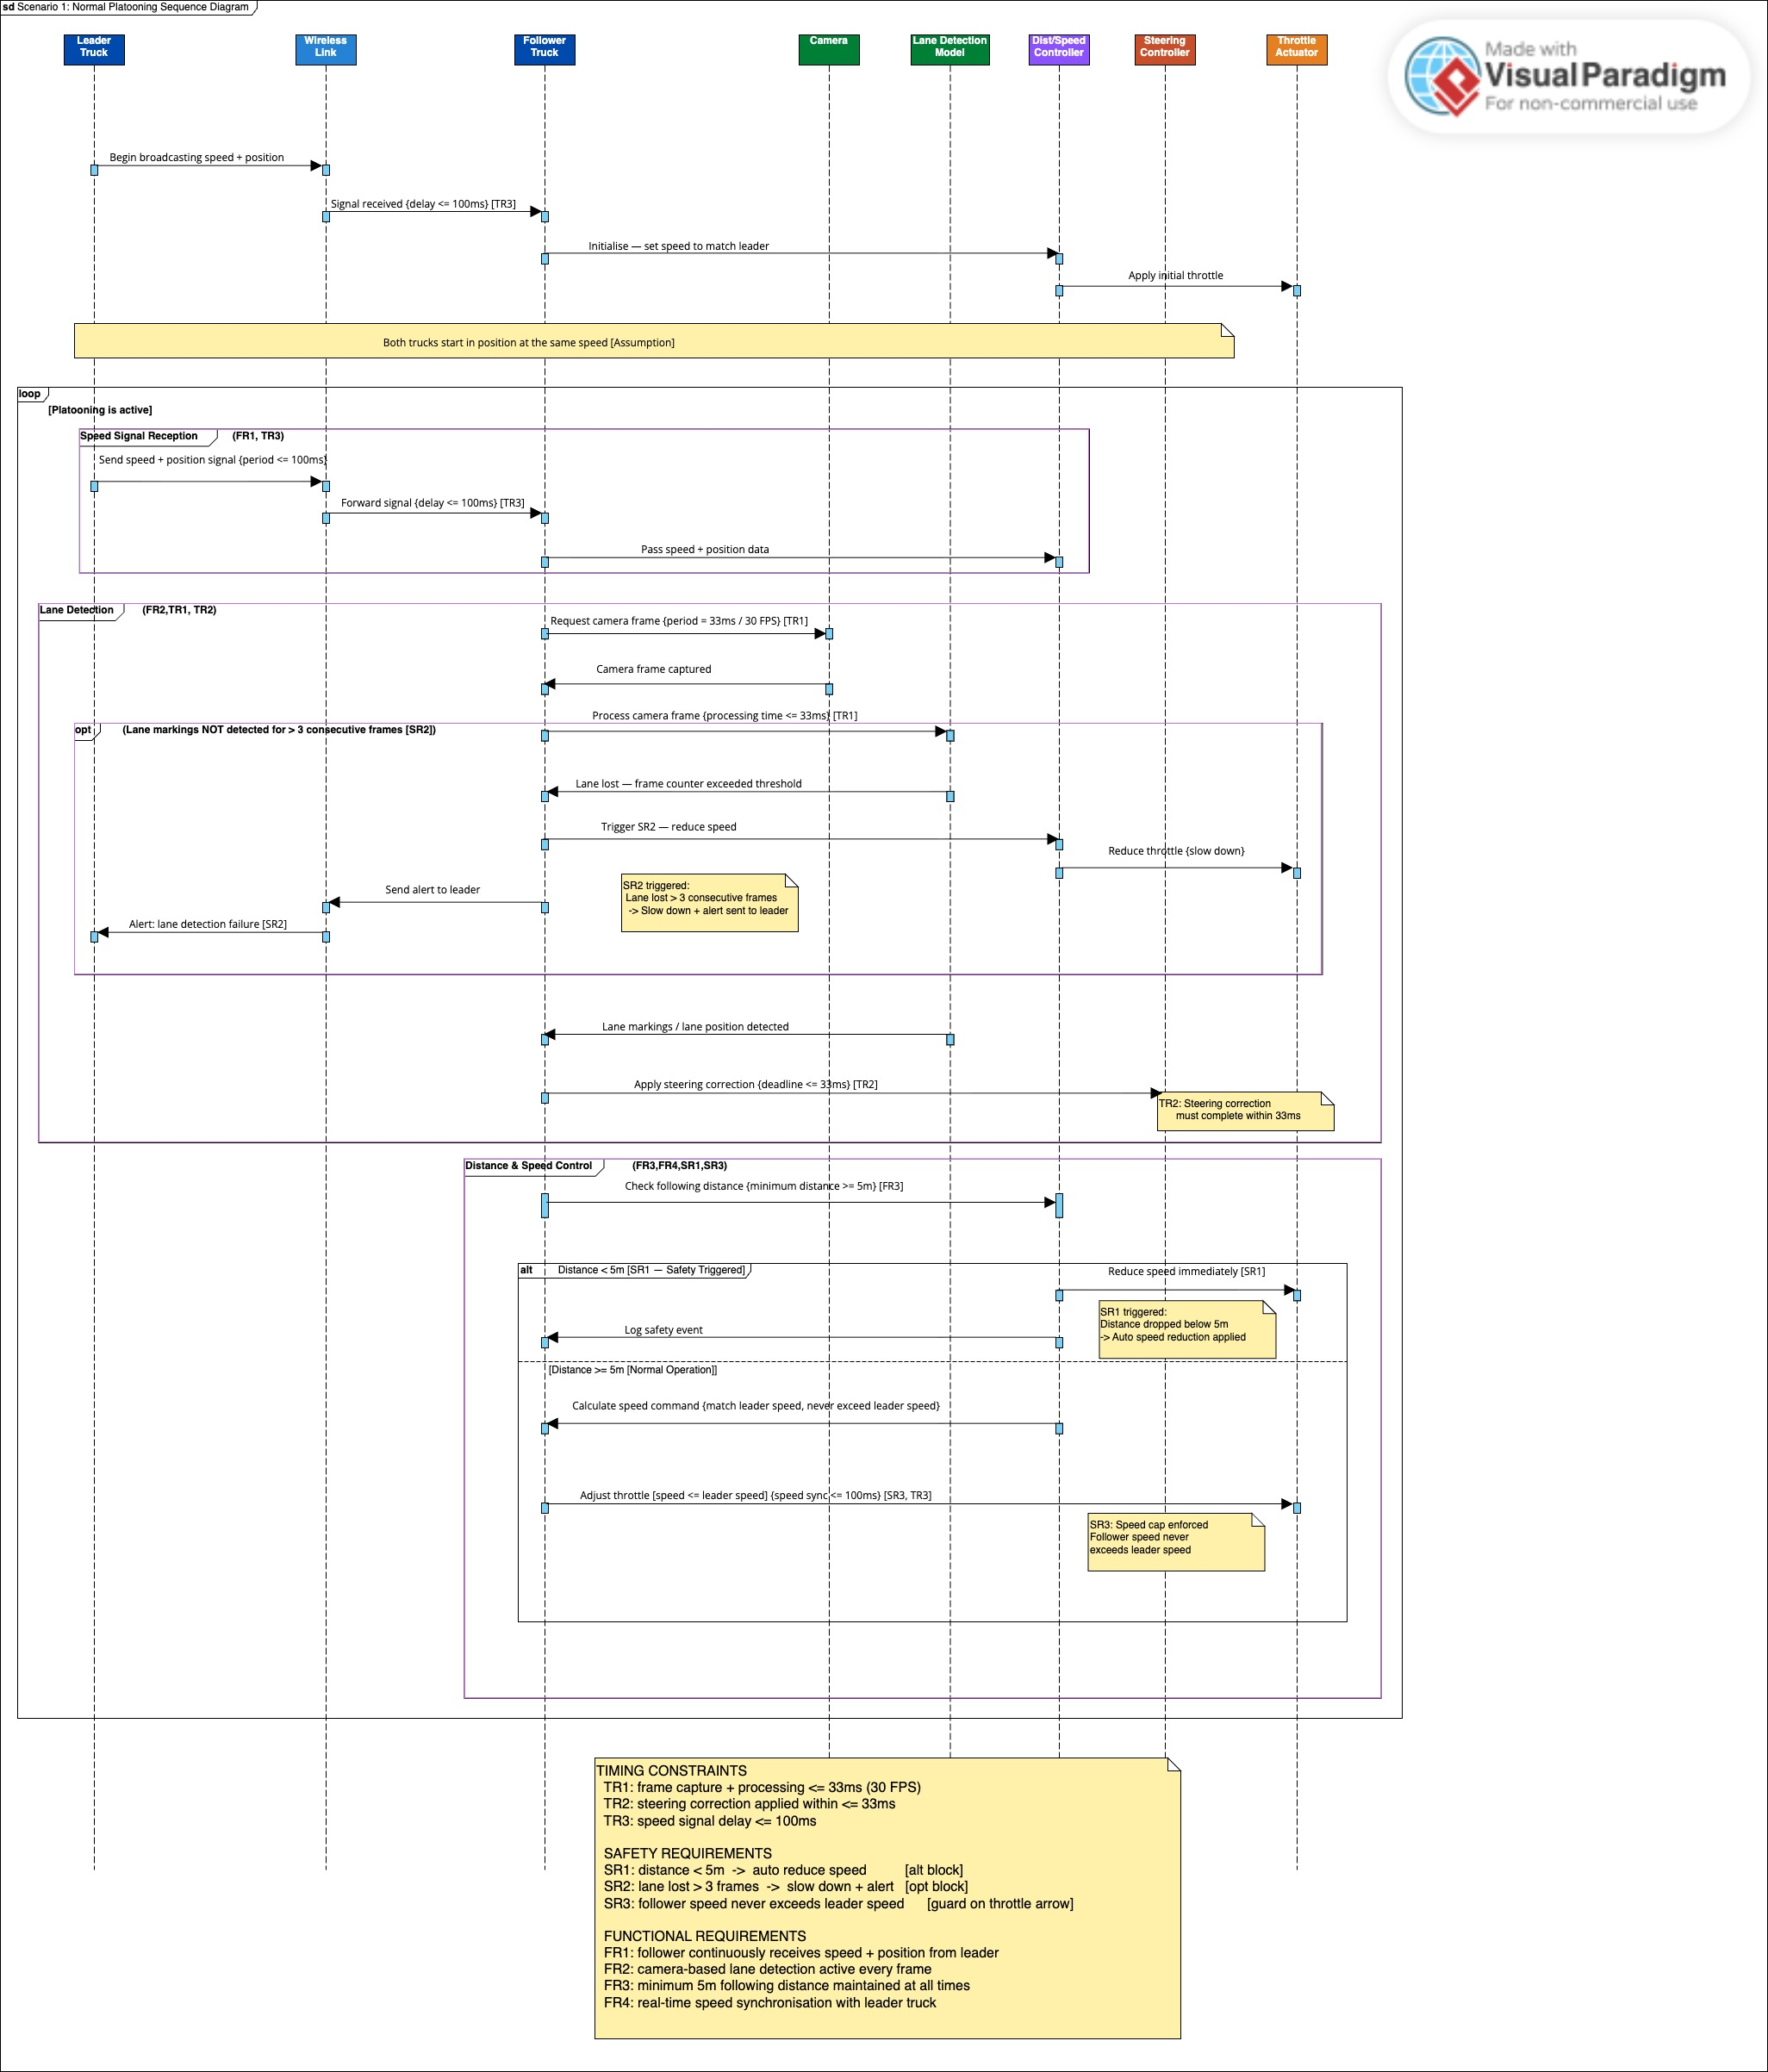
\includegraphics[width=\textwidth]{scen1.jpg}
		\caption{Scenario 1.}
	\end{subfigure}
	\hfill
	\begin{subfigure}[t]{0.32\textwidth}
		\centering
		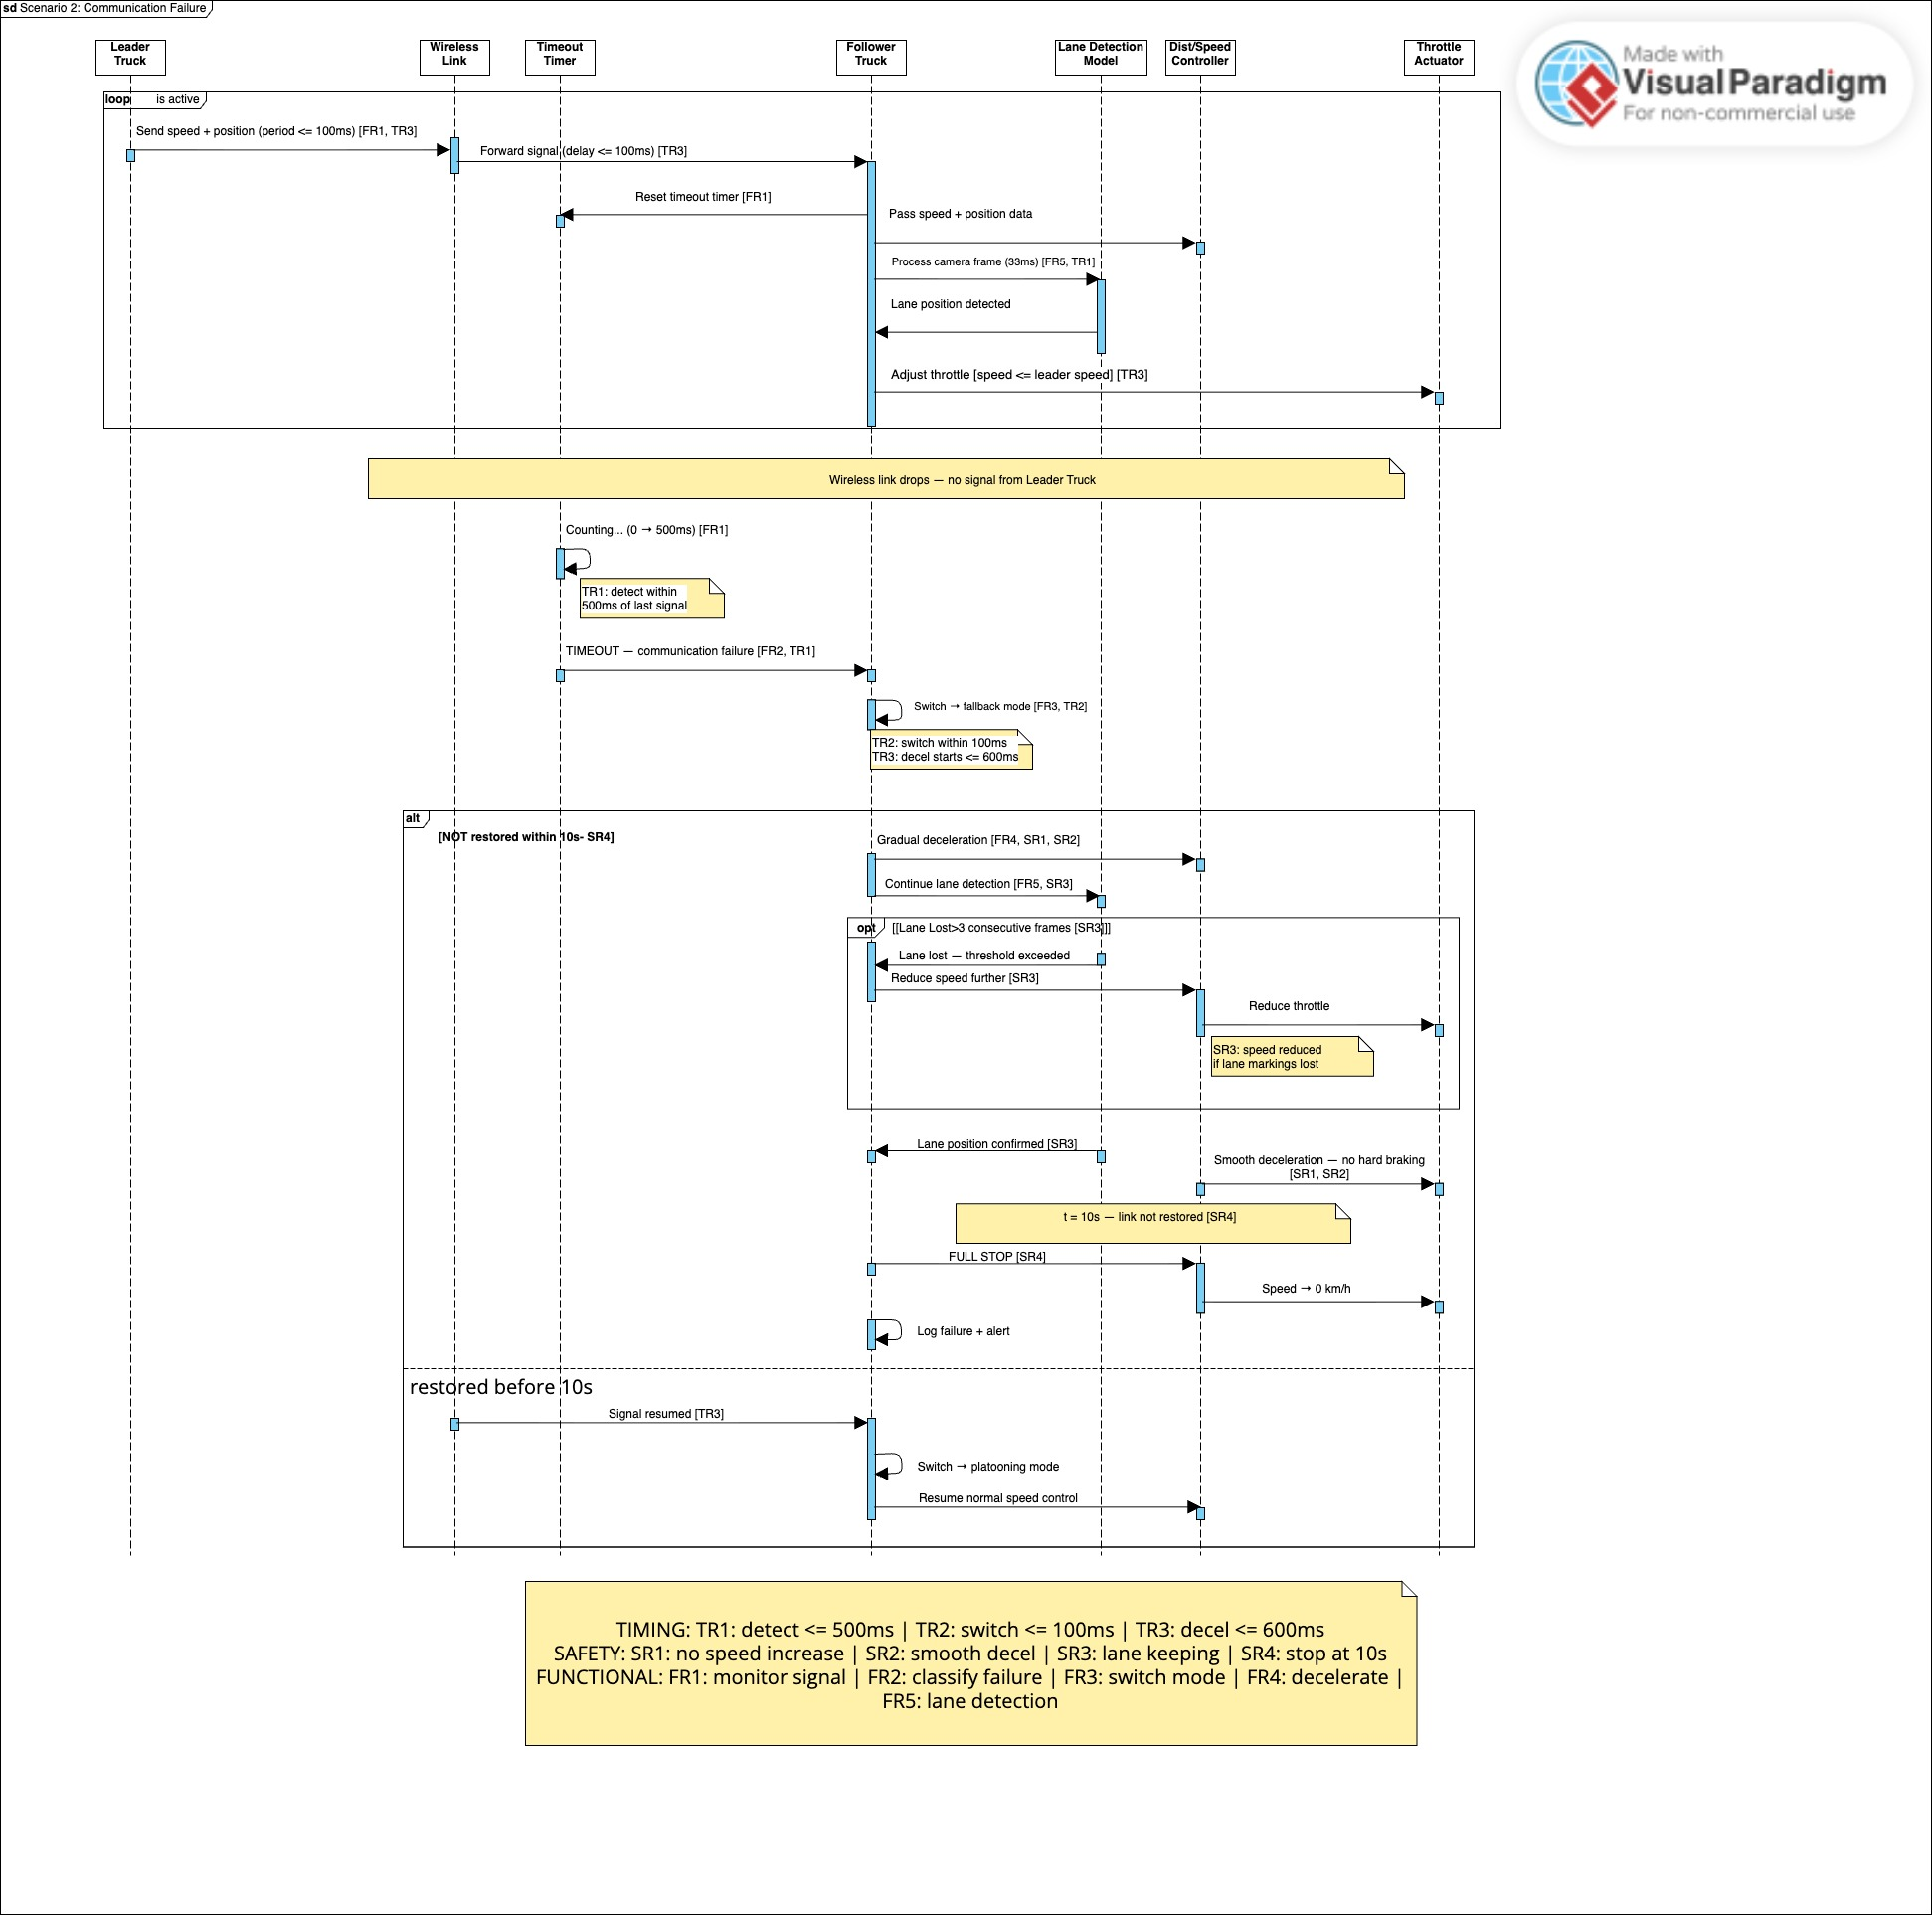
\includegraphics[width=\textwidth]{scen2.jpg}
		\caption{Scenario 2.}
	\end{subfigure}
	\hfill
	\begin{subfigure}[t]{0.32\textwidth}
		\centering
		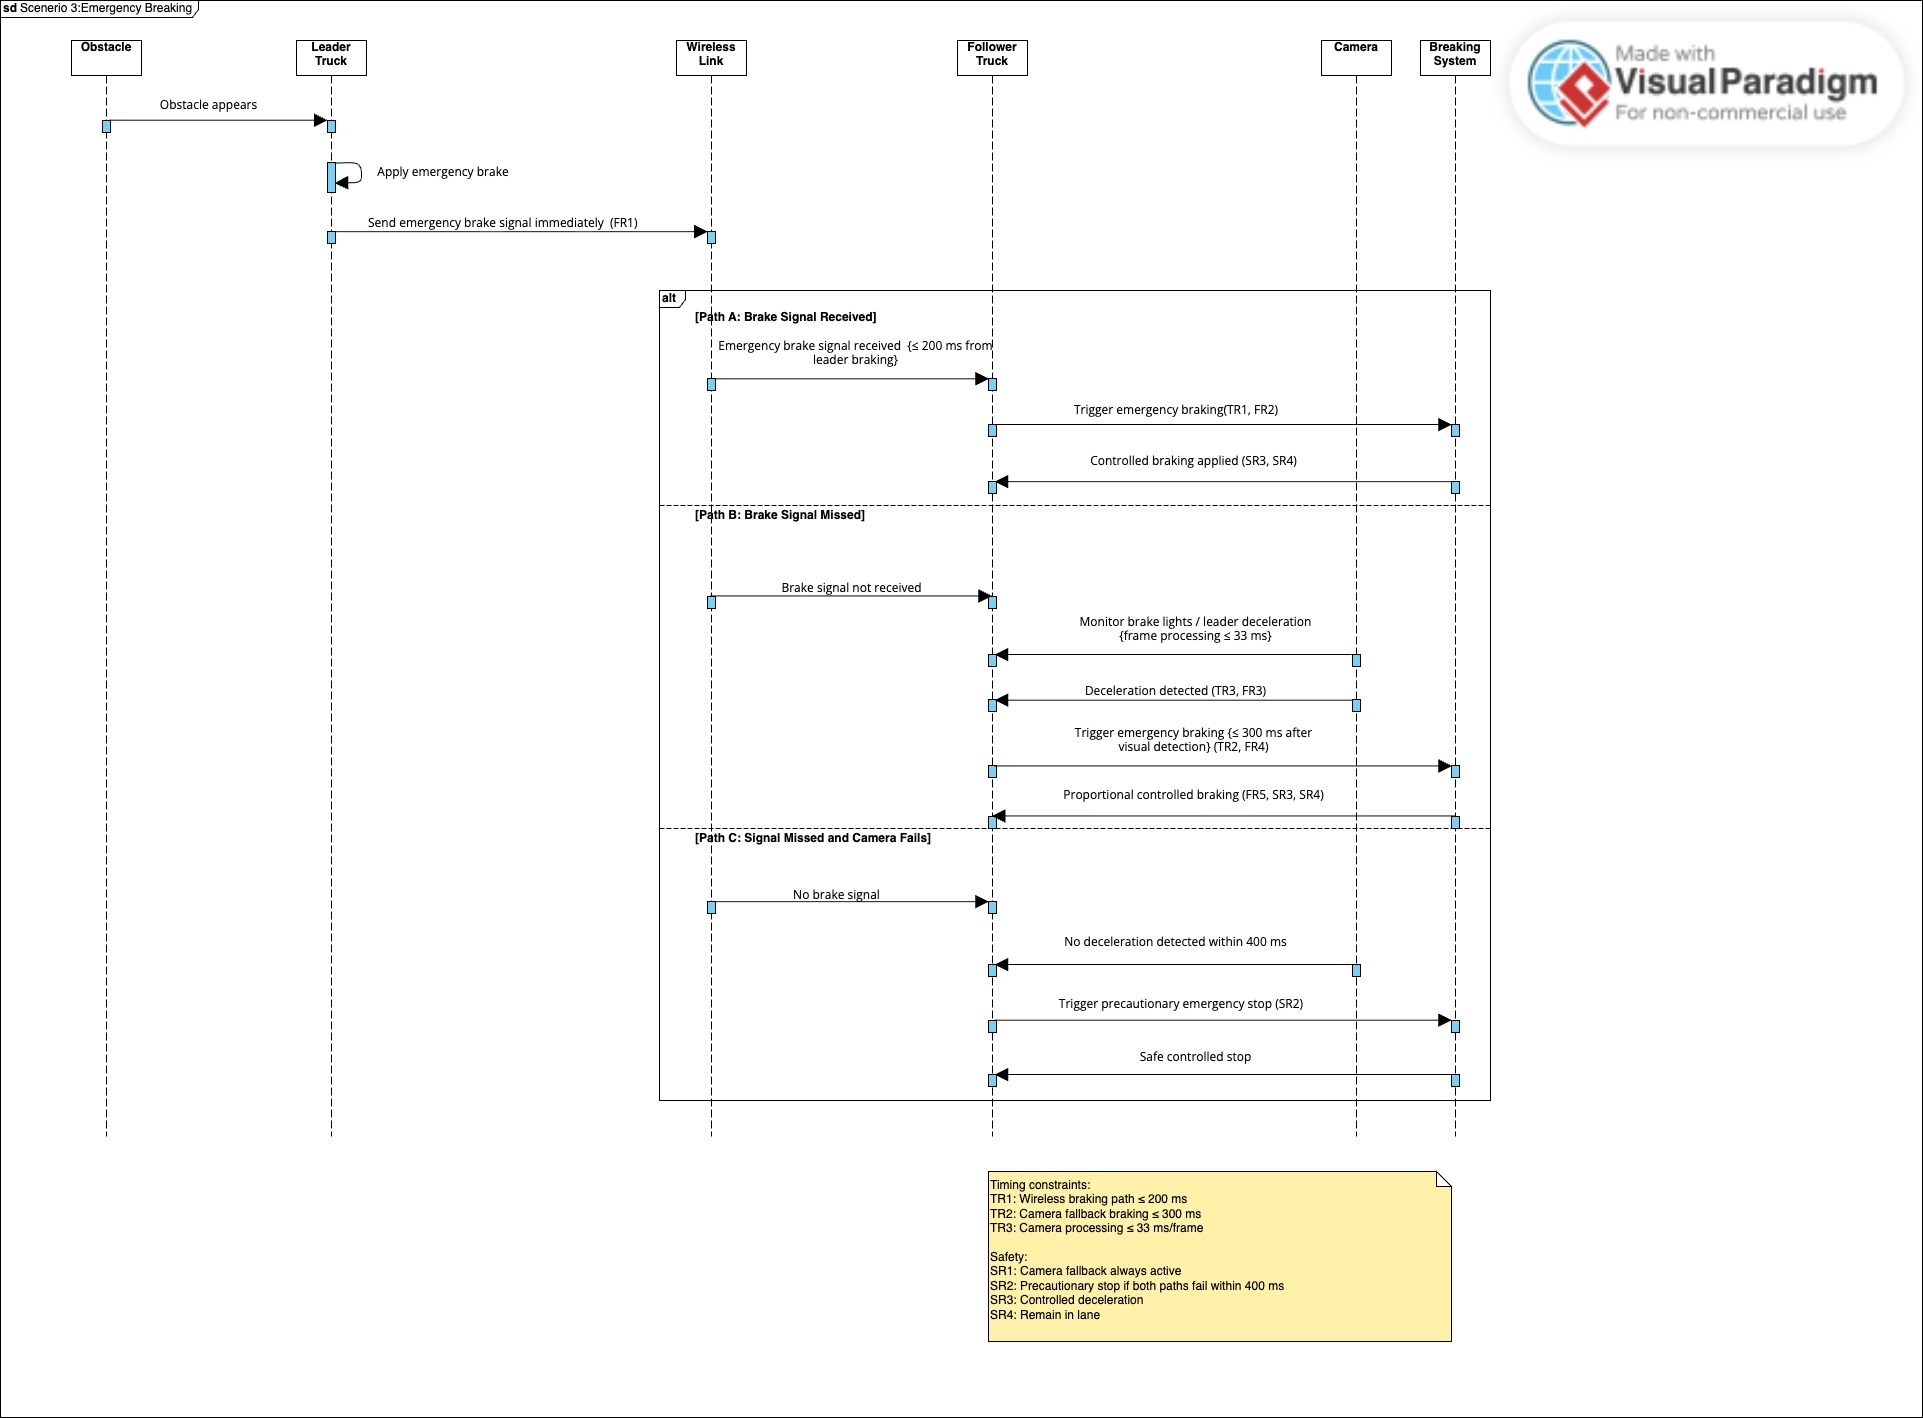
\includegraphics[width=\textwidth]{scen3.jpg}
		\caption{Scenario 3.}
	\end{subfigure}
	\caption{Sequence diagrams for the three scenarios. They show the order of messages between the trucks, the wireless link, the camera, the controllers and the actuators, with the timing constraints written next to the arrows.}
	\label{fig:seq}
\end{figure}

\subsection{Scenario 1 Sequence Diagram}
The first diagram is for normal platooning, so everything is working and the messages just keep repeating in a loop. On each cycle the leader sends its speed and position over the wireless link at least every 100\,ms, and the follower receives this beacon. At the same time the camera captures a frame and the lane detection works out the offset and sends a steering correction within the 33\,ms frame deadline. Alongside this, the distance and speed controller matches the leader's speed if the gap is fine, or sends a reduce-speed command if the gap drops below 5\,m.

\subsection{Scenario 2 Sequence Diagram}
The second diagram shows what happens when the wireless link fails. It starts off like normal platooning, but then the beacons stop arriving. The follower notices this on its own using a timeout, with the 500\,ms detection deadline written next to it, and once the failure is detected it switches into fallback mode within 100\,ms and starts slowing down smoothly. The camera keeps running its lane-keeping loop in parallel, so lane keeping does not stop just because the link is down. The diagram ends with the two possibilities: either a beacon arrives again before 10 seconds and the follower goes back to normal, or the timer runs out and the follower comes to a full stop.

\subsection{Scenario 3 Sequence Diagram}
The third diagram is the emergency, where an obstacle appears in front of the leader. The leader brakes hard and sends a brake signal to the follower, and the diagram shows the three braking paths as alternatives. In Path A the signal gets through and the follower brakes within 200\,ms. In Path B the signal is missed, but the camera sees the leader slowing down and braking is triggered within 300\,ms. In Path C, if neither has happened by 400\,ms, the follower does a precautionary controlled stop. Drawing all three together makes it clear that neither the wireless link nor the camera is a single point of failure.

\section{Timed Automata and UPPAAL Models}
\textit{Written by: Iko-ojo Victor Odaudu}
\\~\\
For the formal side we modelled each of the three scenarios as a network of timed automata in UPPAAL. A timed automaton is basically a small state machine that also keeps track of time using clocks, which lets us describe things like ``this has to happen within 200\,ms''. Once a scenario is modelled, UPPAAL can automatically check properties for us, for example whether the system can ever get stuck, or whether something always happens inside its time limit. The three models are shown in the appendix, in Figures~\ref{fig:m1},~\ref{fig:m2} and~\ref{fig:m3}.

\subsection{Scenario 1 Model}
The first model has three small automata, one for the leader, one for the lane detection, and one for the speed controller, and they talk to each other using channels. The leader sits in a cruising state and keeps sending its signal on a loop. The lane detection cycles through waiting for a frame, processing it, and then either applying steering or raising a lane-lost alert, with a clock and invariant that force each frame to be handled within 33\,ms. The speed controller either reduces speed if the distance is too small, or matches the leader's speed if it is fine. For this model we mainly checked that it is free of deadlock and that the lane-lost alert state can actually be reached.

\subsection{Scenario 2 Model}
The second model has the leader, the follower and the camera. The follower moves through a chain of states, going from platooning, to failure detected, to fallback mode, and finally to a safe stop. It uses two clocks, one that counts the time since the last message and one that runs during fallback. The transition out of platooning fires after 500\,ms with no message, the switch to fallback happens within 100\,ms, and the full stop happens at 10 seconds, with a recovery edge back to platooning if a beacon arrives in time. The camera runs its own loop the whole time, so lane keeping stays active even when the link is down. We checked that the safe-stop state is reachable within the time bound and that the model is free of deadlock.

\subsection{Scenario 3 Model}
The third model has the leader, the follower with its three braking paths, and the camera. The follower can go down Path A after receiving the brake signal, Path B after the camera detects deceleration, or a precautionary stop if neither happened in time, with clocks enforcing the 200\,ms, 300\,ms and 400\,ms deadlines. One design detail worth mentioning is that the leader and the camera each have a small timeout edge, so that if the other side is not ready to receive a message, they carry on anyway instead of waiting forever. This matches reality, since a truck that sees an obstacle should brake whether or not the message got through, and it is also what keeps the model free of deadlock. We checked that each braking path is reachable and that braking always happens inside the 400\,ms worst case.

\section{Combined Control Model (Task 4)}
\textit{Written by: Muhammad Mujhtaba Qaiser}
\\~\\
On top of the three separate scenario models, we built one combined control model that puts the whole system together in UPPAAL. This model has the leader truck, the follower truck, the camera monitor and the environment all in one place, so it covers the distance keeping, the fallback behaviour and the braking at the same time rather than in separate pieces. The point of this model is to check the system as a whole, and not just one situation at a time. The model is shown in the appendix, in Figure~\ref{fig:m4}.

This combined model passes all of its verification queries, seventeen of them in total, which between them cover the distance keeping, the fallback behaviour and the braking. The most important one for safety is that the distance between the trucks can never drop below the minimum, which is written as \texttt{A[] dist >= D\_MIN}. The \texttt{A[]} part means ``on all paths, at all times'', so this is a strong claim: it proves that in every possible run of the model, no matter how the timing works out, the follower never gets closer to the leader than the safe distance, so the two trucks can never crash into each other. The rest of the queries are a mix of reachability checks, which confirm that the useful states like fallback and safe stop can actually happen, and safety checks that make sure the bad states never do. Just like the scenario models, it was also checked to be free of deadlock.

\section{Scalable Combined Model}
\textit{Written by: Hany Chowdhury}
\\~\\
The combined model in the previous section only describes a single follower behind the leader. A real platoon though can have several followers in a row, so we also built a scalable version of the combined model. The reason for having it is that safety in a convoy is not automatically the same thing as safety for one pair of trucks, because each follower has to keep its distance from the truck right in front of it, and we wanted to prove the safe-distance guarantee for the whole line and not just for one gap. The model is shown in the appendix, in Figure~\ref{fig:m4s}.

The way it works is that the parts of the system are turned into templates that get instantiated once for each follower, and the important variables become arrays that are indexed by the truck number. So instead of a single \texttt{dist}, \texttt{comm\_ok} or \texttt{svm\_bad}, the model uses \texttt{dist[i]}, \texttt{comm\_ok[i]} and \texttt{svm\_bad[i]}, and the environment, lane detection and controller automata (\texttt{env0}, \texttt{lane0}, \texttt{ctrl0}) exist once for each index \texttt{i}. This means that adding another truck to the platoon does not change the logic at all, it only adds another instance, and the same behaviour, timing and transitions apply to it. Because the safety property is written over the array, the query \texttt{A[] dist[i] >= D\_MIN} then proves that no follower anywhere in the convoy ever gets closer than the safe minimum distance to the truck ahead of it. The scalable model is checked to be free of deadlock as well.

\section{Simulation and Verification Results}
\textit{Written by: Iko-ojo Victor Odaudu}
\\~\\
We used UPPAAL's simulator to step through each model and watch the system move through its states, which was a good way to check that the models behave the way we intended before actually running the formal checks. For the verification itself, each model was checked against a set of queries, mainly safety properties (``this must always hold'') and reachability properties (``this state can be reached''), where the reachability ones were used to confirm that safe states like fallback and safe stop can actually be reached.

For all three scenarios, and for both the combined and the scalable models, the checks passed. This includes the query \texttt{A[] not deadlock}, which is the proof that the system can never reach a state where it is stuck with nothing to do, and the safe-distance property \texttt{A[] dist >= D\_MIN} for the whole system. The results for the combined model and the scalable model are shown in the appendix, in Figure~\ref{fig:verif}, where every query is marked as satisfied.

\section{Limitations}
\textit{Written by: Muhammad Mujhtaba Qaiser}
\\~\\
There are a few limitations that we are aware of. On the machine learning side, the balanced dataset is quite small at around 104 samples per class, so having more real data would make the model more robust, and the whole approach depends on the green line being visible and the lighting being reasonable. It also relies on the single offset feature, so if the line detection is off, then the prediction suffers as well.

On the formal side, the UPPAAL models are simplified on purpose. Speed and distance are represented as states or single variables rather than real physics, so the models prove the logic and the timing, but not the exact dynamics of a real truck. Some of the requirements are built into the structure of the model rather than being checked with their own query, and the camera is modelled as a fixed loop instead of something that only fires on a real change. These simplifications are pretty normal for this kind of modelling, but they are still worth keeping in mind.

\section{Responsibility Matrix}
Table~\ref{tab:resp} shows who was mainly responsible for each part. A lot of the parts were worked on together, especially the machine learning pipeline, but the table lists the main owner of each task.

\begin{table}[H]
	\centering
	\caption{Responsibility matrix for Team 5.}
	\label{tab:resp}
	\begin{tabular}{lll}
		\hline
		\textbf{Task} & \textbf{Main responsibility} & \textbf{Notes} \\
		\hline
		Data collection (ScienceTruck) & Muhammad Mujhtaba Qaiser & Gathering training data \\
		SVM model training & Iko-ojo Victor Odaudu & Feature, pipeline, tuning \\
		Testing on ScienceTruck & Hany Chowdhury & Live testing of the model \\
		Scenario definitions & All members & One scenario each \\
		Sequence diagrams (SysML/UML) & Hany Chowdhury & All three diagrams \\
		Timed automata / UPPAAL (Task 3) & Iko-ojo Victor Odaudu & All three scenario models \\
		Combined control model (Task 4) & Muhammad Mujhtaba Qaiser & Full single-follower system \\
		Scalable combined model & Hany Chowdhury & Parameterized for N followers \\
		Report and presentation & All members & Shared \\
		\hline
	\end{tabular}
\end{table}

\section{Conclusion}
Putting both sides together, the project produced a follower truck that stays on the line using the camera and the SVM, keeps a safe distance, and reacts safely when things go wrong. The line following model reached about 99\% accuracy on the balanced data and runs live on the truck. On the formal side, all three scenario models, the combined control model and the scalable combined model were verified, every timing bound held, and every model was proven free of deadlock. The combined and scalable models also proved that the safe minimum distance is never broken, which is the core safety guarantee for platooning, and the scalable model takes that guarantee from a single follower and stretches it out to a whole convoy. Overall the project shows how a self-driving behaviour can be built with machine learning and, at the same time, backed up with a formal proof that it behaves safely.

\section{Declaration of Originality}

We, Iko-ojo Victor Odaudu, Hany Chowdhury and Muhammad Mujhtaba Qaiser, herewith declare that we have composed the present paper and work by ourselves and without the use of any other than the cited sources and aids. Sentences or parts of sentences quoted literally are marked as such; other references with regard to the statement and scope are indicated by full details of the publications concerned. The paper and work in the same or similar form have not been submitted to any examination body and have not been published. This paper was not yet, even in part, used in another examination or as a course performance. We agree that our work may be checked by a plagiarism checker. \\~\\

\paragraph{AI tools we have used:}

\begin{itemize}
	\item Claude AI was used to help  proofread this report (didnt accept all its recomendations) and to help with understanding upaal and finding online tutorials.
	Image generator (Gemini) was used only to create the illustration images of the platooning scenarios in the presentation slides.
\end{itemize}

\hspace*{\fill}\begin{tabular}{@{}l@{}}\hline
	\makebox[10cm]{Date\&Place - Team 5}
\end{tabular}

\nocite{*}
\printbibliography

\appendix
\section{Appendix: UPPAAL Models and Verification Results}
This appendix collects the UPPAAL screenshots referenced in the main text: the timed automata models for the three scenarios, the combined and scalable control models, and the verification results.

\begin{figure}[H]
	\centering
	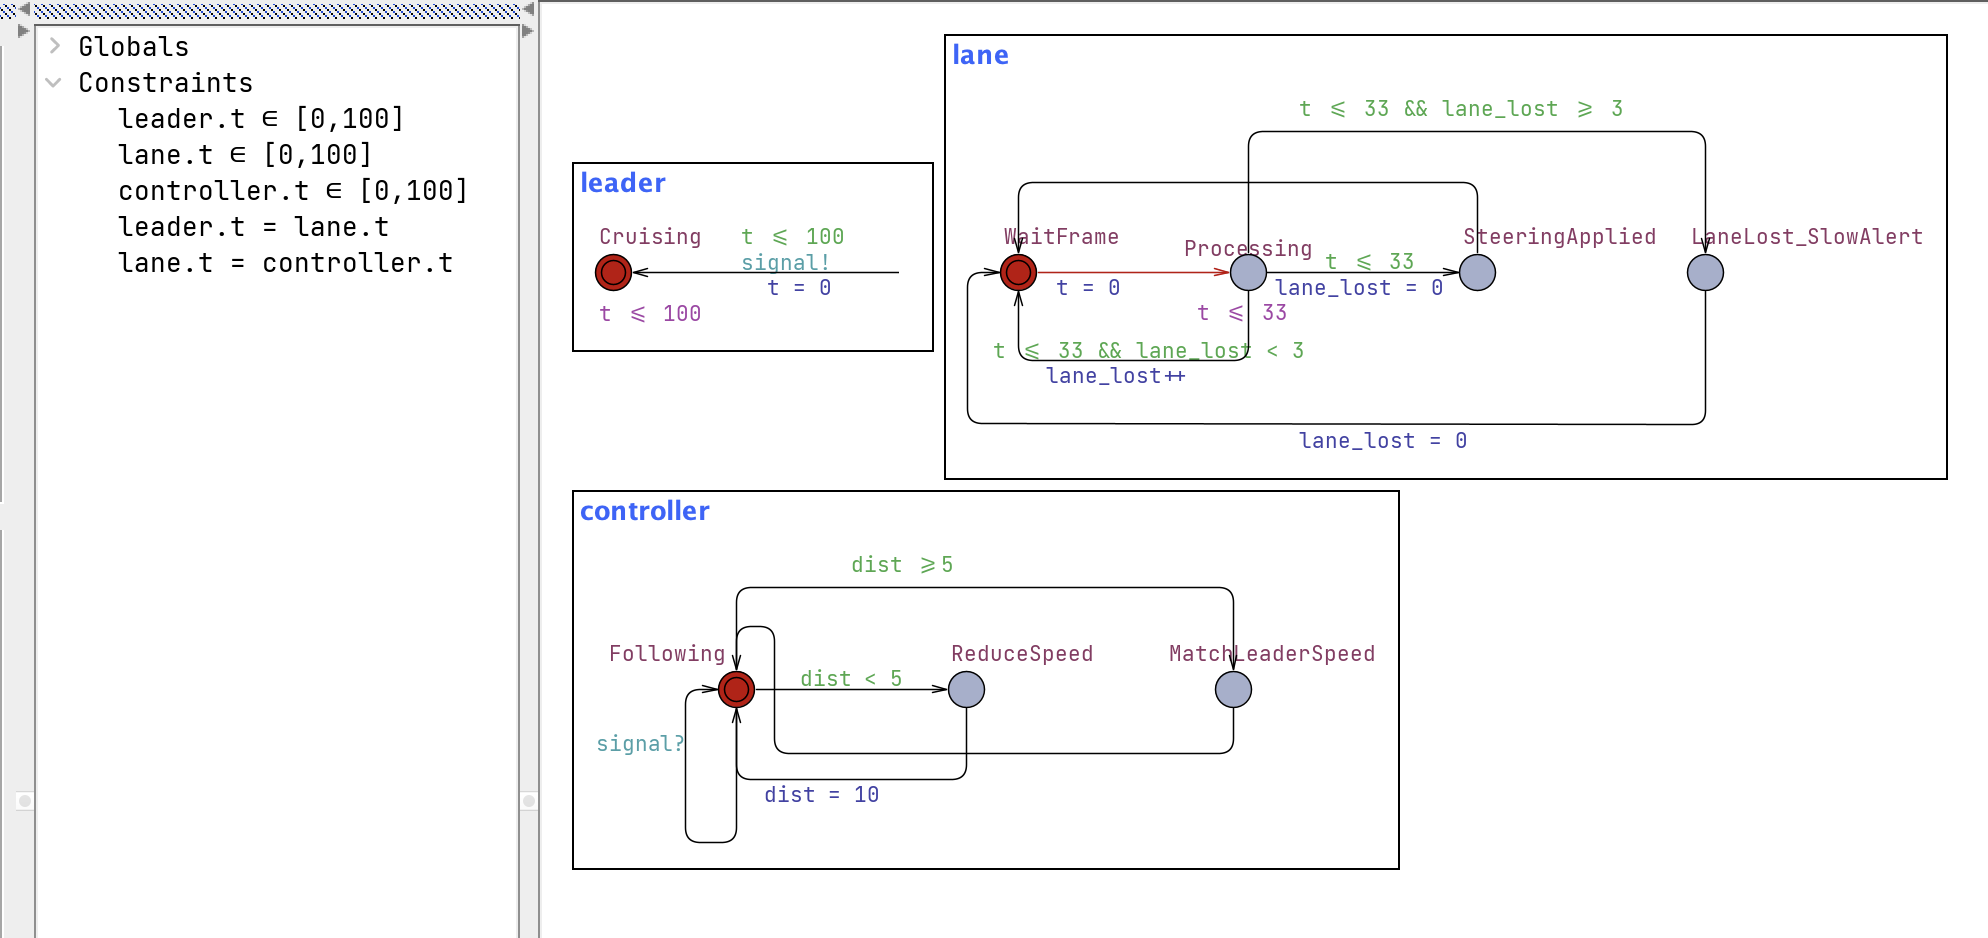
\includegraphics[width=0.72\textwidth]{1_model.png}
	\caption{UPPAAL model for Scenario 1: leader, lane detection and speed controller.}
	\label{fig:m1}
\end{figure}

\begin{figure}[H]
	\centering
	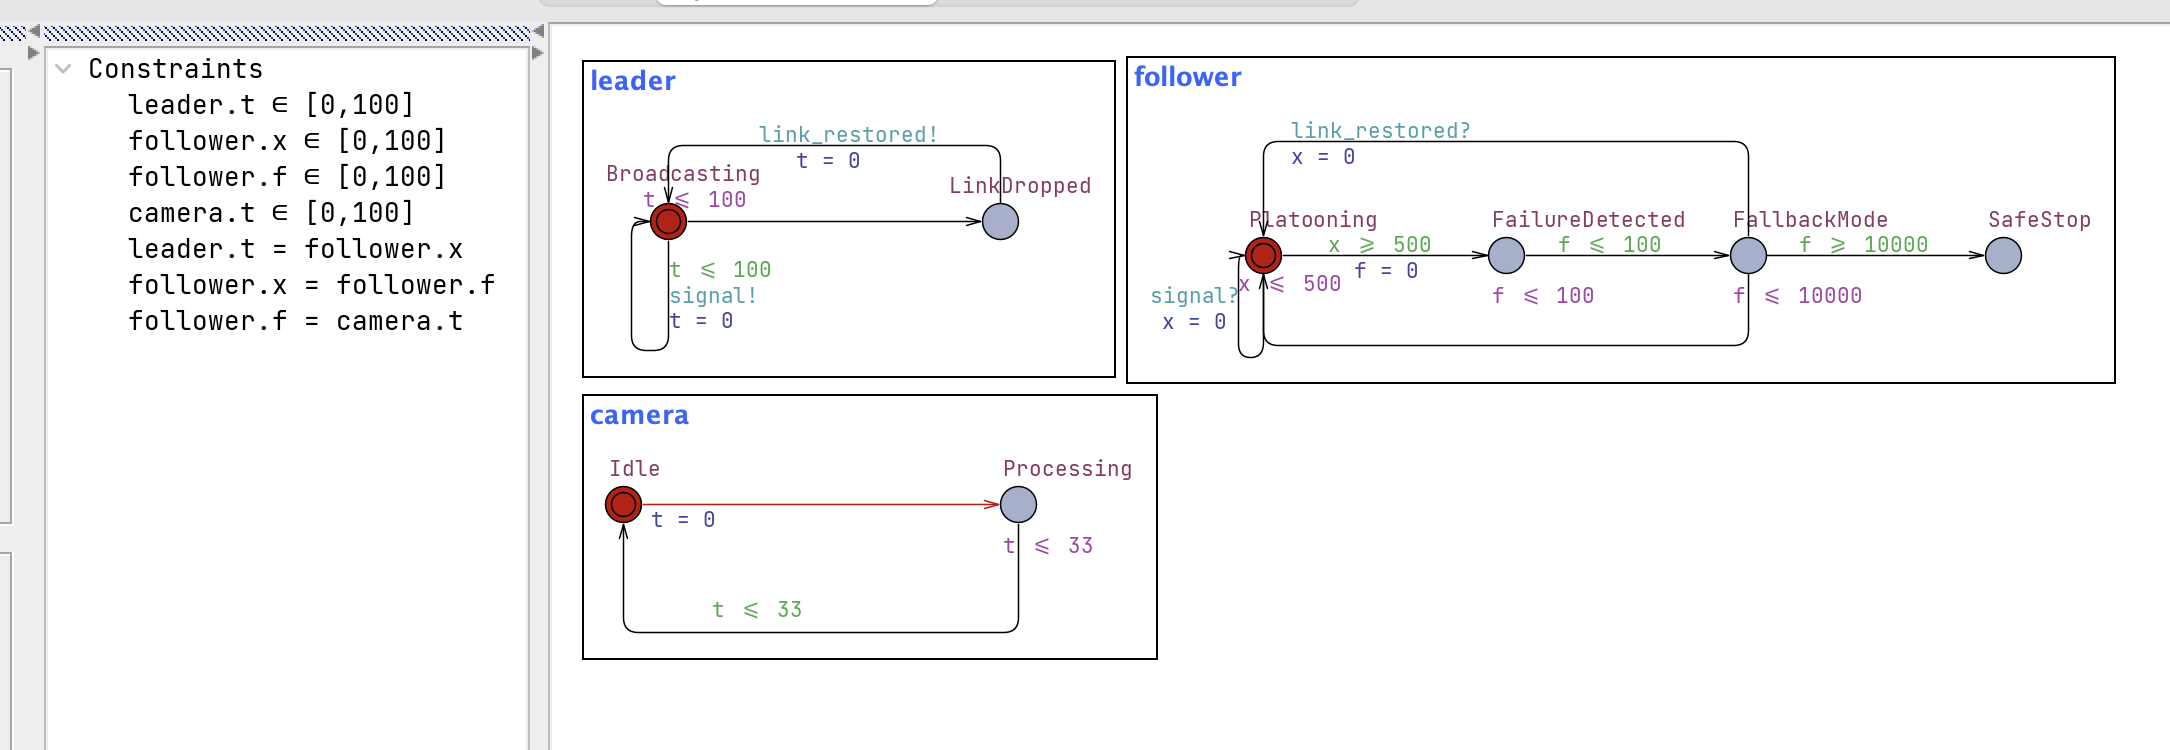
\includegraphics[width=0.72\textwidth]{2_model.png}
	\caption{UPPAAL model for Scenario 2: the follower detects the timeout and moves through fallback to a safe stop, while the camera keeps running.}
	\label{fig:m2}
\end{figure}

\begin{figure}[H]
	\centering
	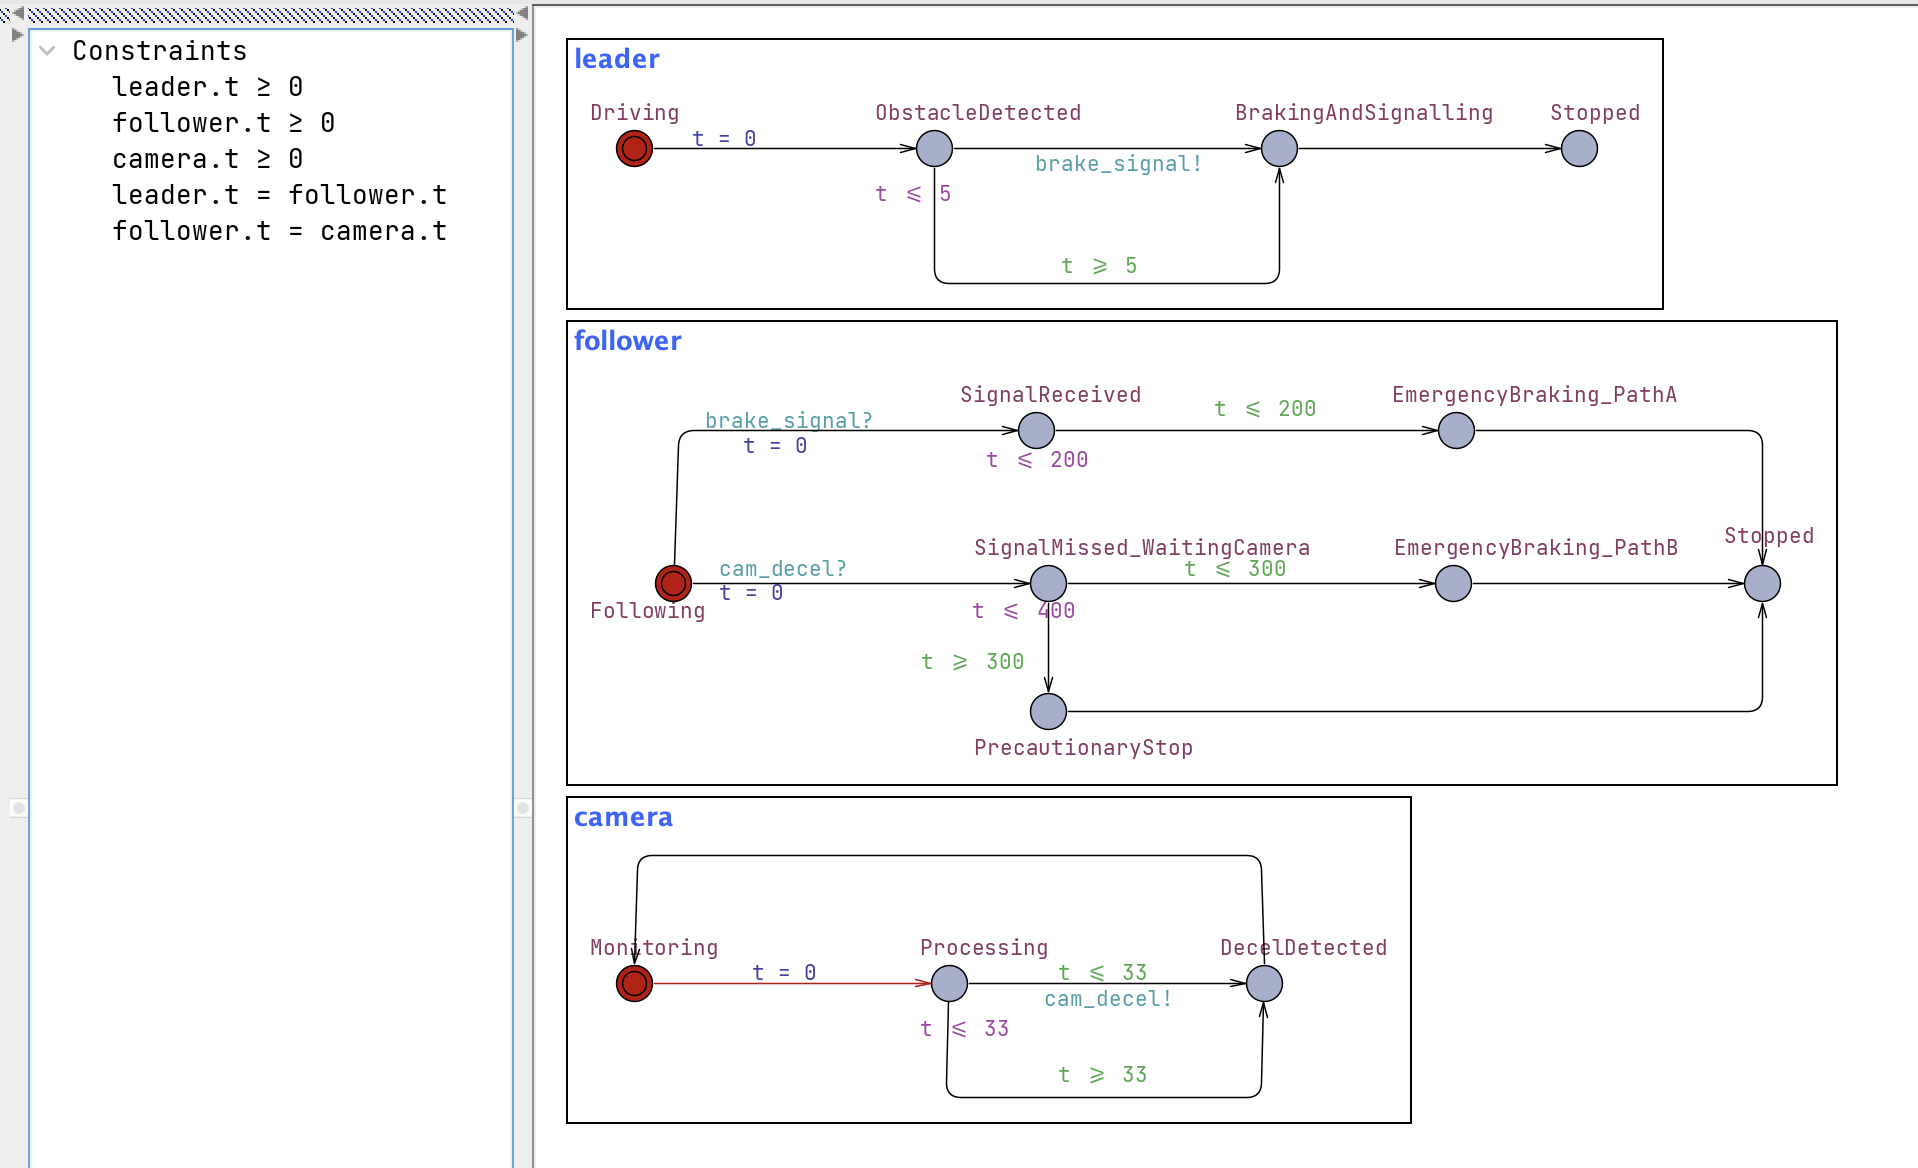
\includegraphics[width=0.72\textwidth]{3_model.png}
	\caption{UPPAAL model for Scenario 3: the follower has three independent braking paths so that neither the signal nor the camera is a single point of failure.}
	\label{fig:m3}
\end{figure}

\begin{figure}[H]
	\centering
	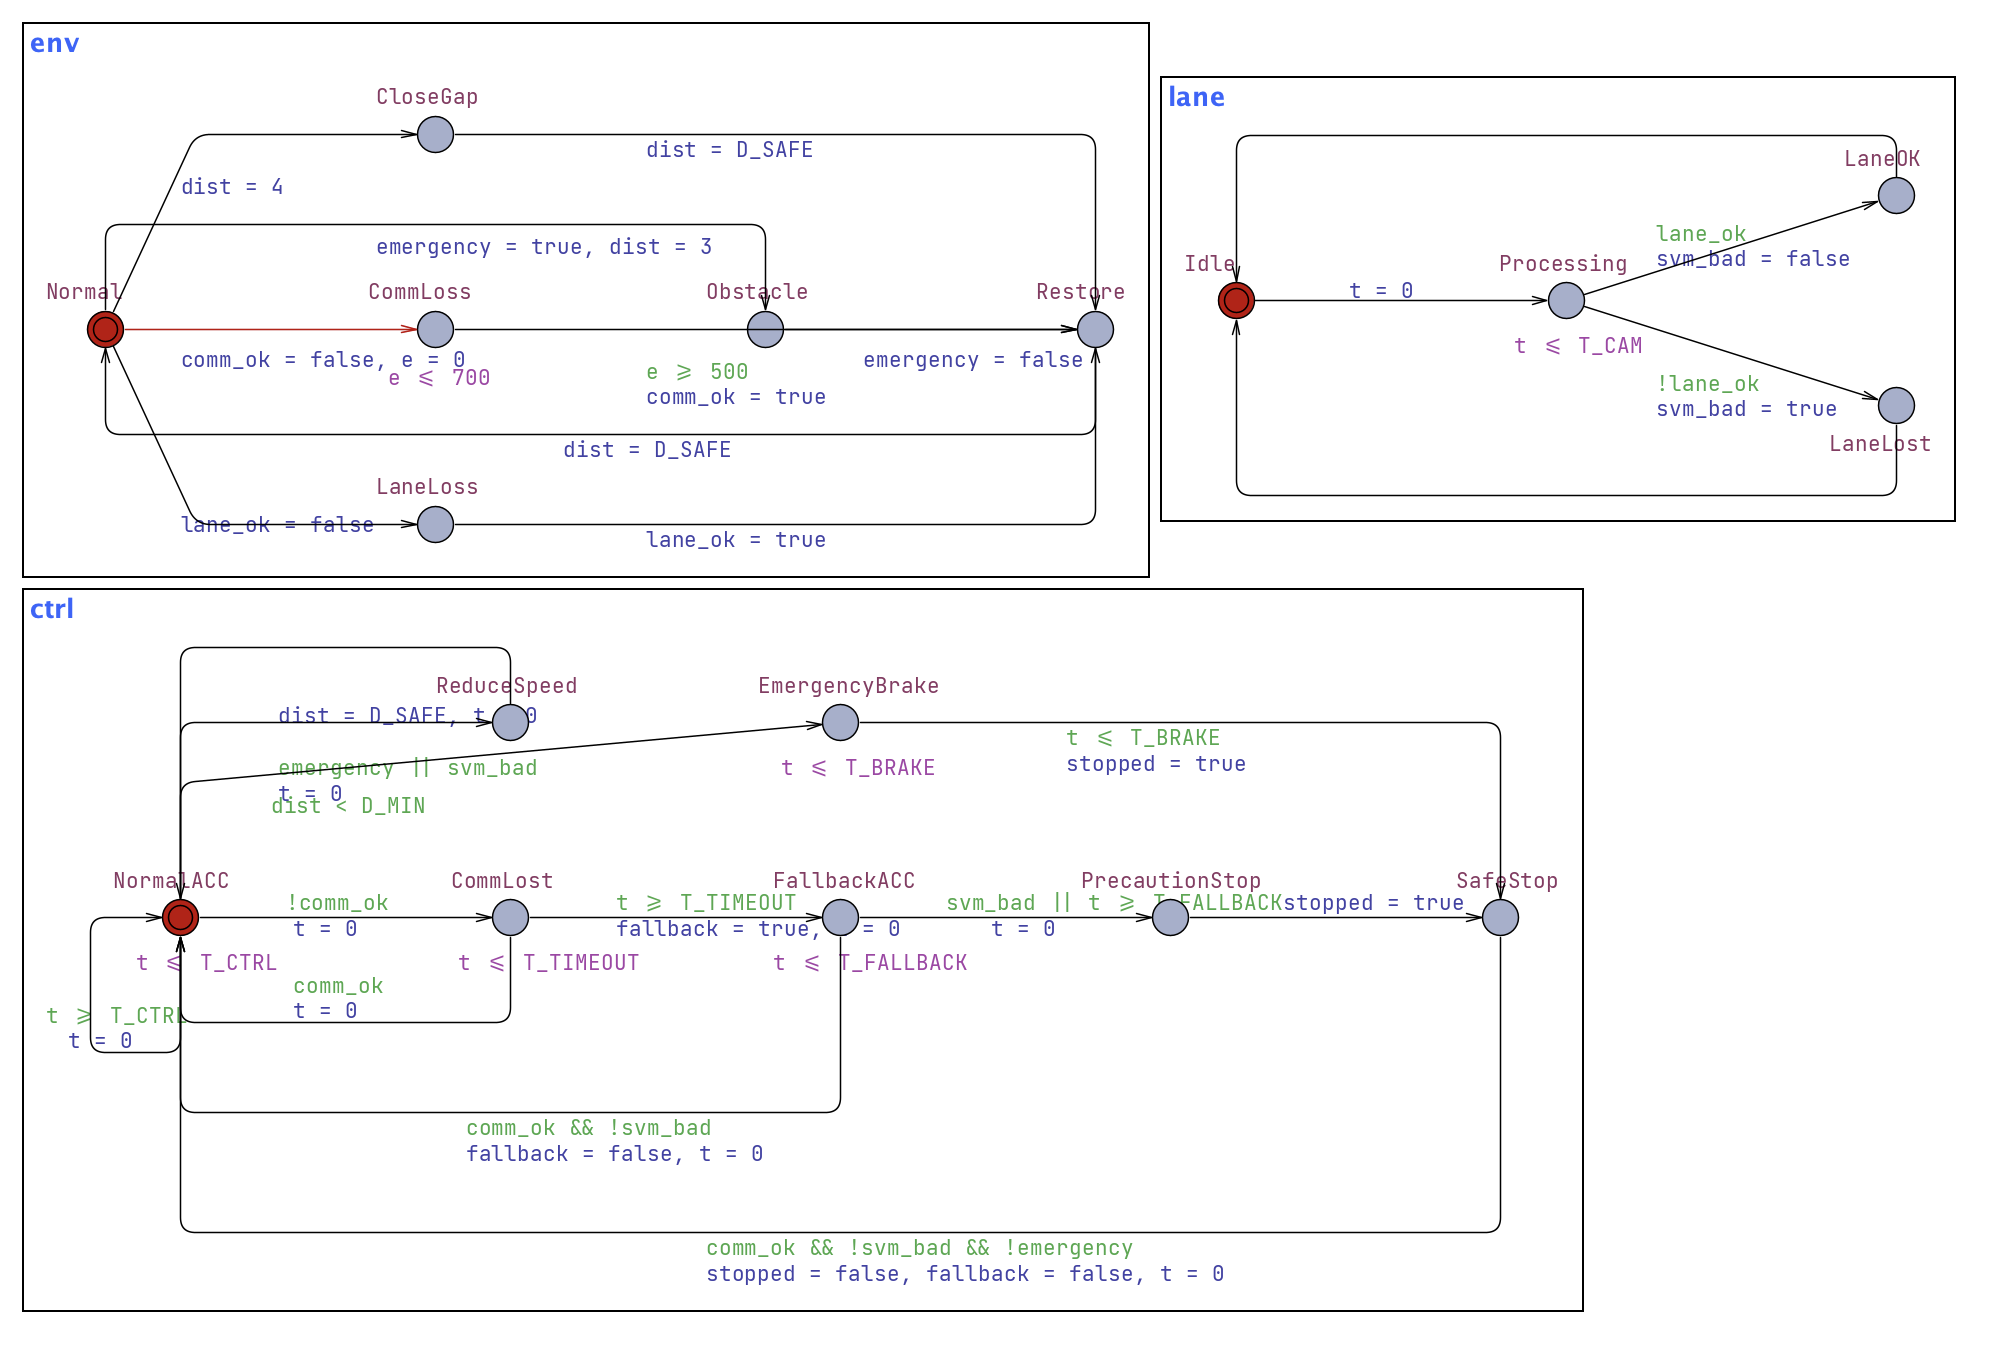
\includegraphics[width=0.72\textwidth]{4_model.png}
	\caption{Combined control model: leader, follower, camera monitor and environment in a single UPPAAL model covering distance keeping, fallback and braking together.}
	\label{fig:m4}
\end{figure}

\begin{figure}[H]
	\centering
	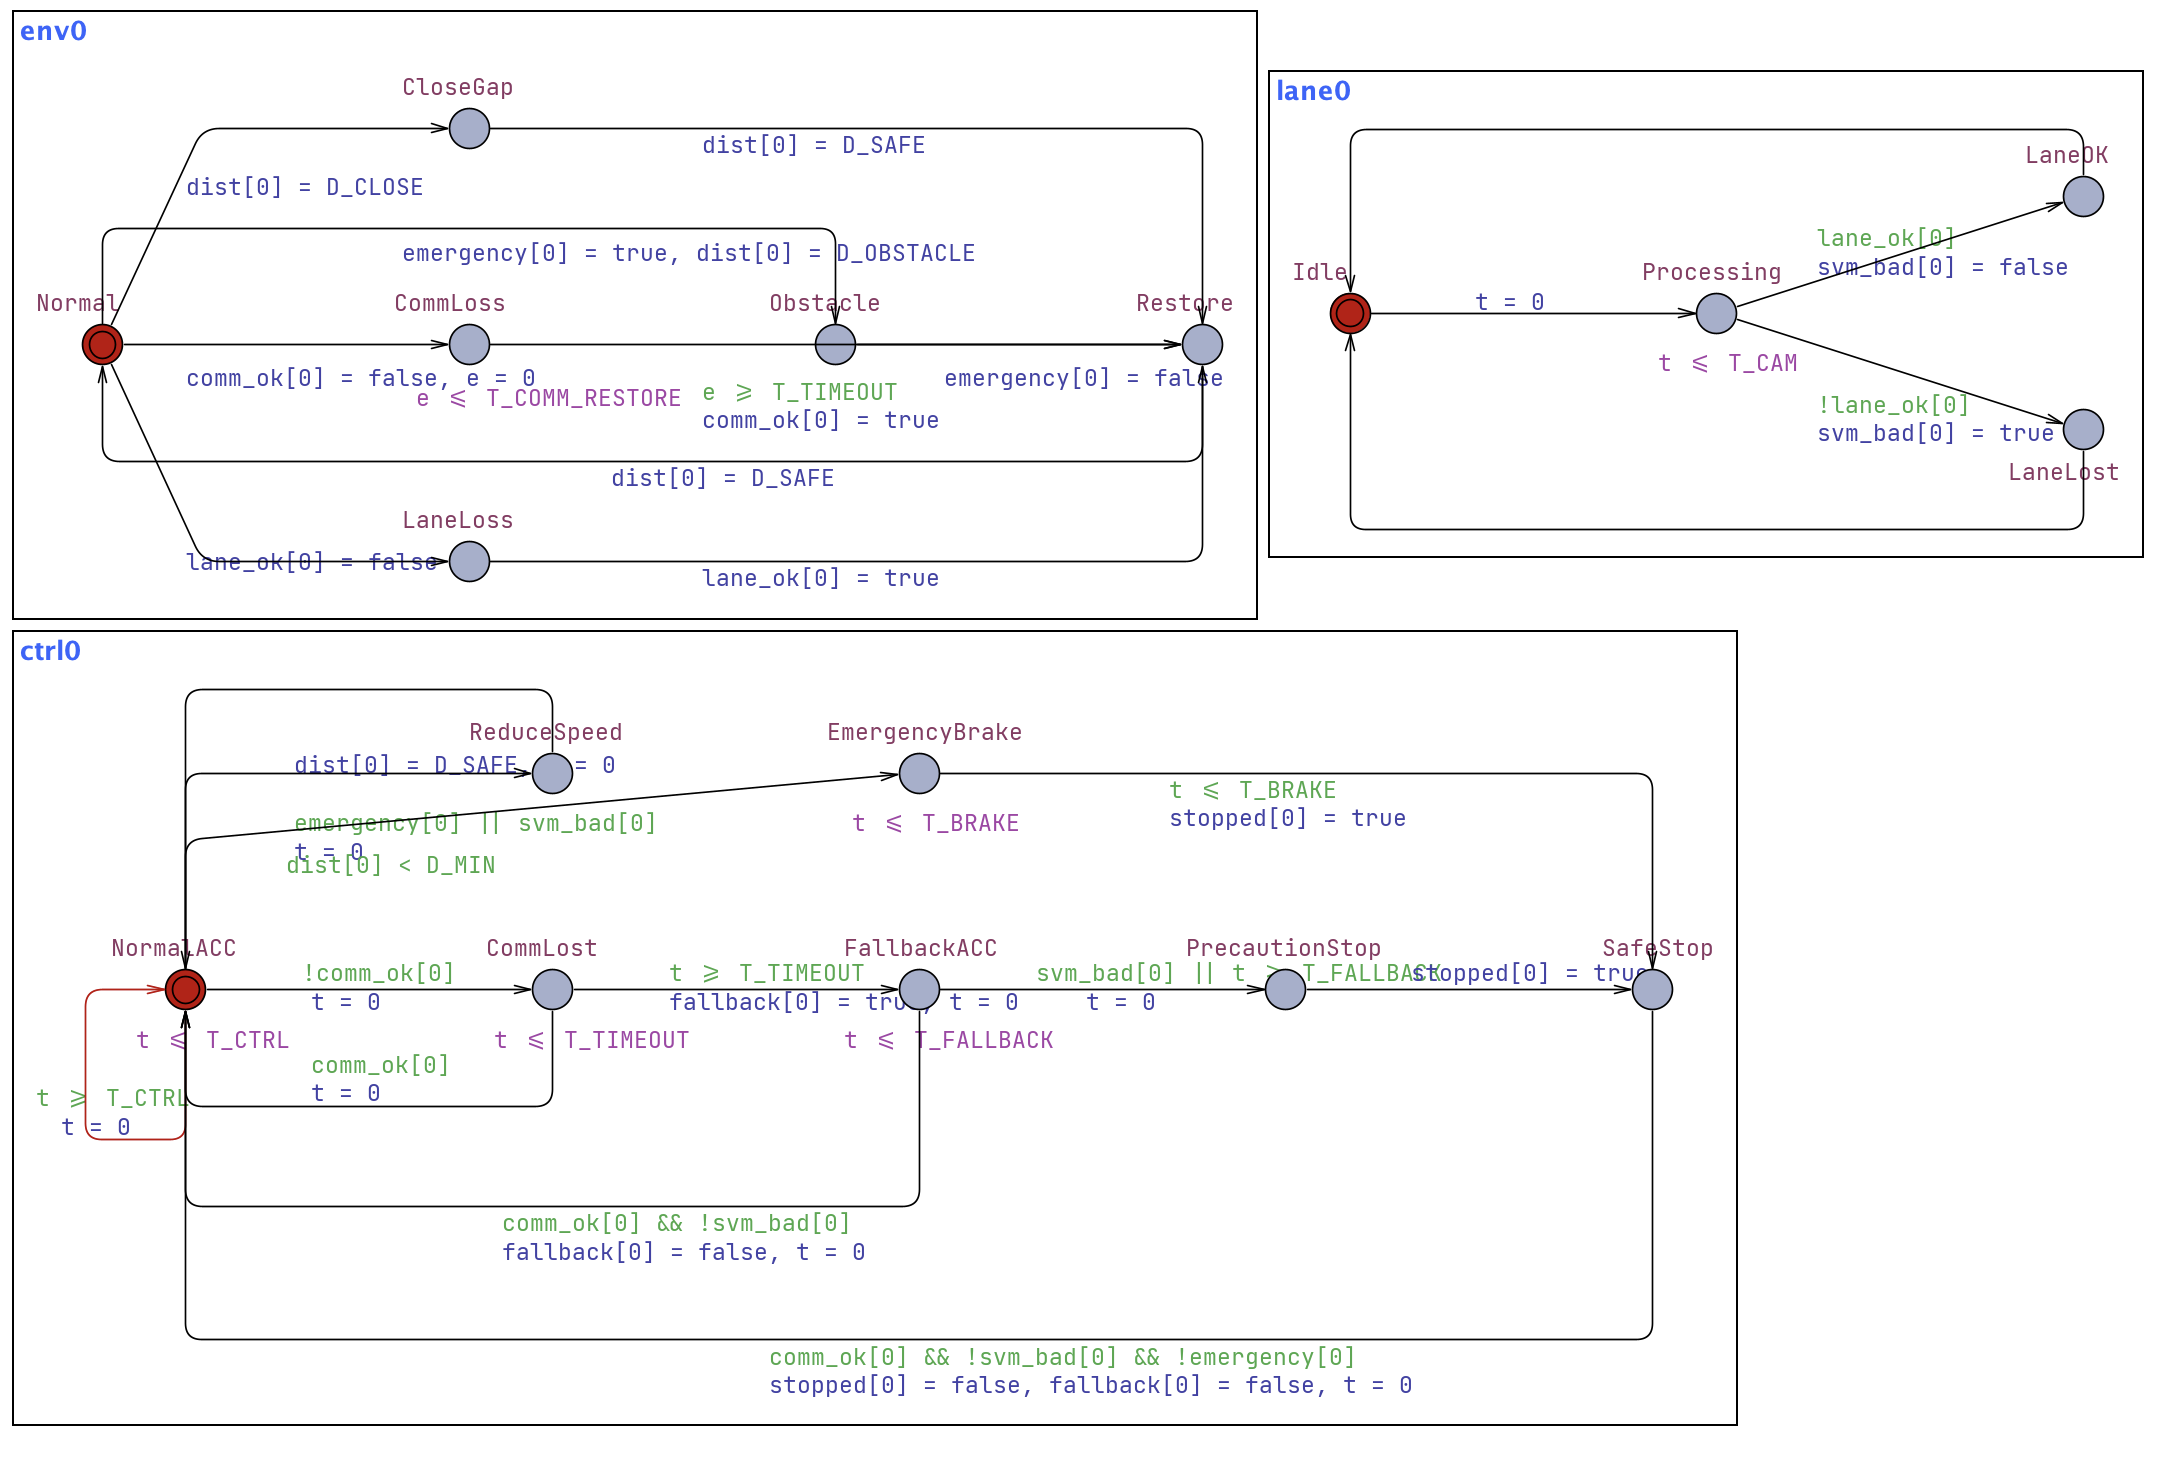
\includegraphics[width=0.8\textwidth]{4_scaled_model.png}
	\caption{Scalable combined model. The environment, lane detection and controller are templates instantiated per follower, with array-indexed variables (\texttt{dist[i]}, \texttt{comm\_ok[i]}, \texttt{svm\_bad[i]}), so the same safety guarantee extends to a platoon of several trucks.}
	\label{fig:m4s}
\end{figure}

\begin{figure}[H]
	\centering
	\begin{subfigure}[t]{0.48\textwidth}
		\centering
		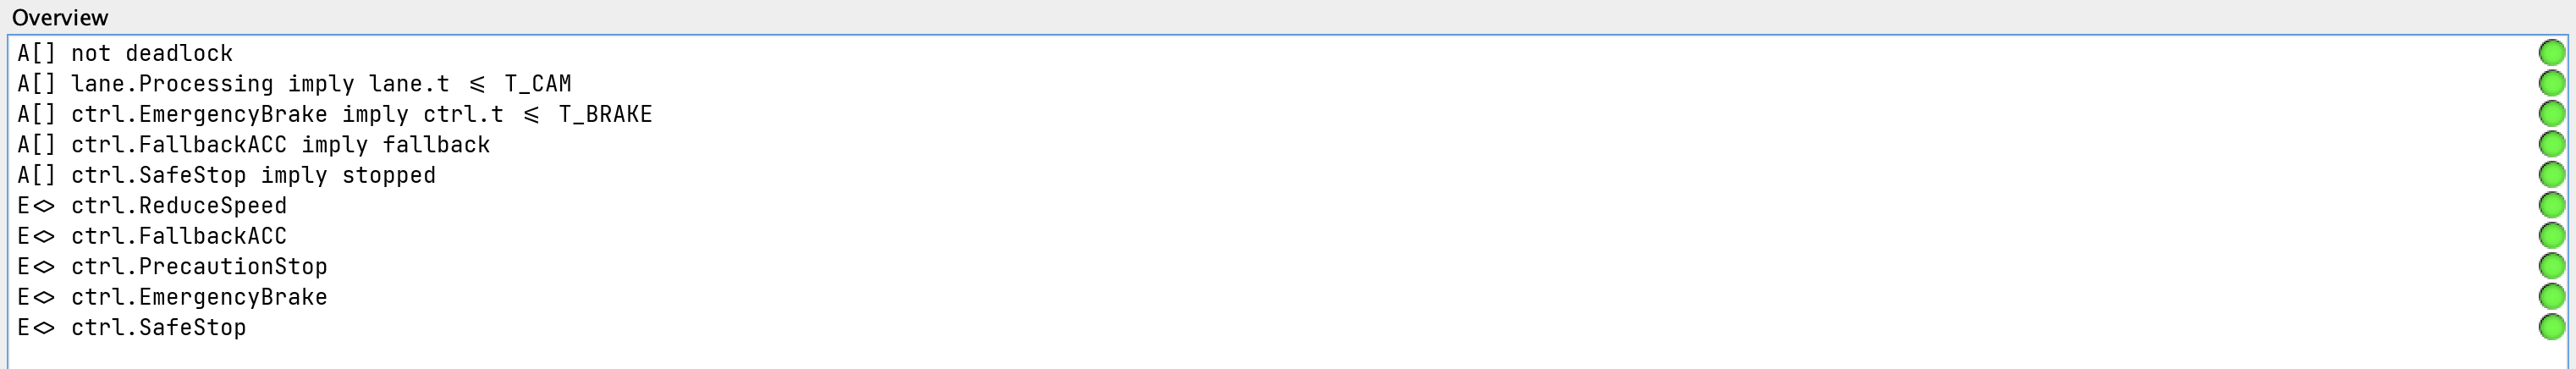
\includegraphics[width=\textwidth]{4_verif.png}
		\caption{Combined control model.}
	\end{subfigure}
	\hfill
	\begin{subfigure}[t]{0.48\textwidth}
		\centering
		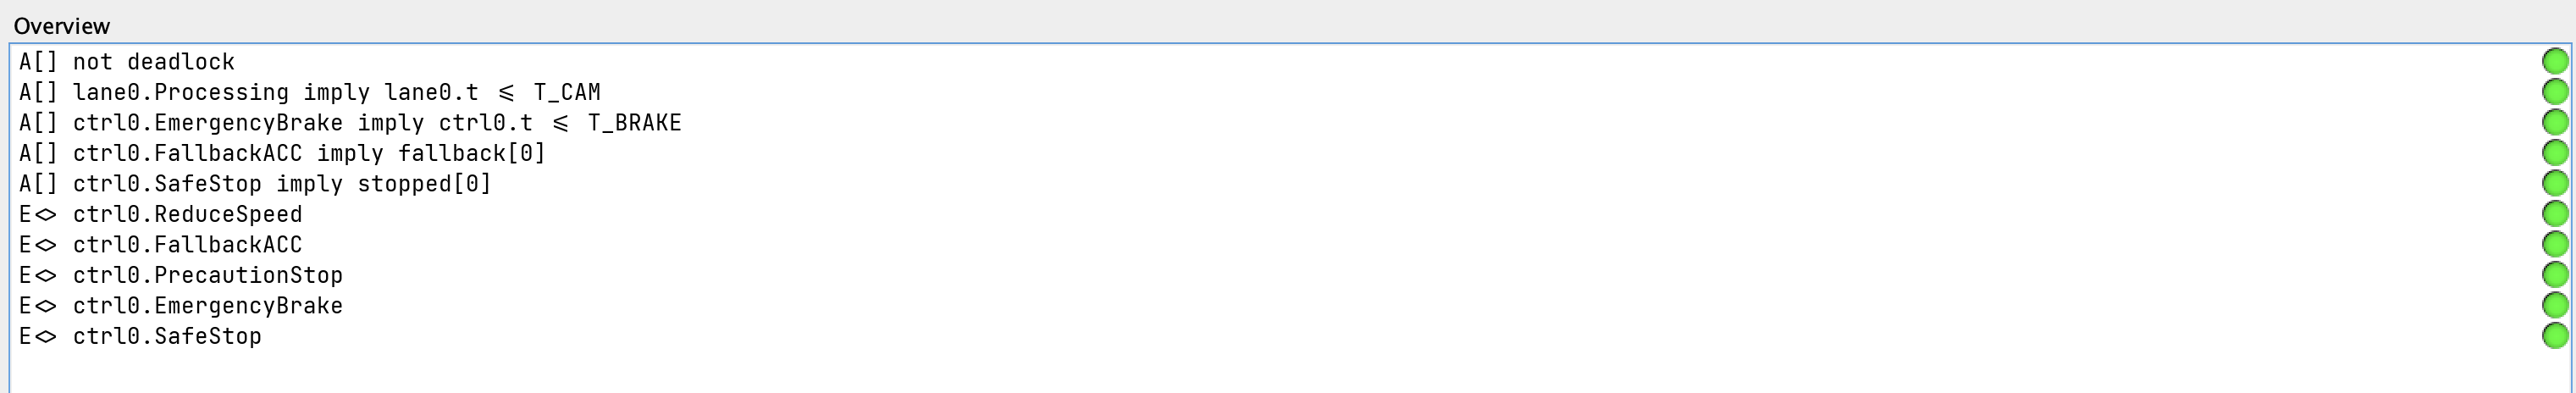
\includegraphics[width=\textwidth]{4_scaled_model_verif.png}
		\caption{Scalable combined model.}
	\end{subfigure}
	\caption{Verification results for the combined and scalable models. Every query is satisfied, including \texttt{A[] not deadlock} (deadlock freedom) and the safe-distance property.}
	\label{fig:verif}
\end{figure}

\end{document}
